
\section{The \pkg{sbtools} package}
\begin{itemize}
	\item{Goal to allow programmatic access to core SB functionality}
	\item{Harmonize the SB data structures with common R interfaces}
	\item{Lightweight R package that can be quickly added to existing projects and shared broadly}
\end{itemize}


%code example
% \begin{example}
  % x <- 1:10
  % result <- myFunction(x)
% \end{example}

\subsection{Data access API}
The data access functionality of \pkg{sbtools} makes it easy to 
access any public item's data, attached files and metadata. All items
in ScienceBase have a unique identifier that can be used to directly 
access specific items. 

\begin{example}
> test_item = item_get("4f4e4b24e4b07f02db6aea14")
> test_item
<ScienceBase Item> 
  Title: Coastal-change and glaciological maps of Antarctica
  Creator/LastUpdatedBy:      / 
  Provenance (Created / Updated):  2010-10-06T04:25:43Z / 2014-07-21T17:45:42Z
  Children: FALSE
  Item ID: 4f4e4b24e4b07f02db6aea14
  Parent ID: 4f4e4771e4b07f02db47e1e4
\end{example}

For convenience, \pkg{sbtools} defines an \code{sbitem} object, which is 
returned by \pkg{sbtools} functions when referencing objects. The underlying
data structure is a list. All available metadata for an item can be listed
and accessed in the same way as a named list.

\begin{example}
> names(test_item) 
 [1] "link"              "relatedItems"      "id"               
 [4] "identifiers"       "title"             "citation"         
 [7] "provenance"        "hasChildren"       "parentId"         
[10] "contacts"          "webLinks"          "browseCategories" 
[13] "browseTypes"       "tags"              "dates"            
[16] "facets"            "files"             "distributionLinks"
[19] "previewImage"     

> item_get(test_item)$citation
[1] "Geological Survey (U.S.), 1999-08-05, Coastal-change 
and glaciological maps of Antarctica:  Fact SheetCoastal-change and 
glaciological maps of Antarctica."
\end{example}

On ScienceBase, all items are organized in a tree structure, with one 
parent and potentially many children. \pkg{sbtools} allows the user to 
easily traverse the tree structure. For example, in some projects, the hierarchy has 
important meaning. For other projects, it may relates to the user or
organizational owner of the data.

\begin{example}
#parent ID always available as item attribute
> parent = item_get(test_item$parentId)
> parent
  Title: USGS Publications Warehouse
  Creator/LastUpdatedBy:      / 
  Provenance (Created / Updated):  2012-02-29T15:42:41Z / 2014-07-08T21:42:20Z
  Children: TRUE
  Item ID: 4f4e4771e4b07f02db47e1e4
  Parent ID: 4f4e4771e4b07f02db47e1da
  
#getting sibling items
> item_list_children(parent)
[1] "55b98fbee4b08f6647be5179" "541d45a4e4b0f68901ec30ef"
[3] "55b361b3e4b09a3b01b5daad" "53516ef9e4b05569d8059f34"
[5] "4f4e4ab2e4b07f02db66f5e3" "5351704ee4b05569d805a2e4"
\end{example}

ScienceBase items may have data or metadata files attached to them. 
You can list and download attached files directly using \pkg{sbtools}.

\begin{example}
#returns files attached to item
item_list_files(test_item)
#returns local path to downloaded files
item_file_download(test_item, dest_dir = tempdir())
\end{example}

ScienceBase has special functionality when certain data types are 
stored. One example is spatial data. When spatial data are properly 
tagged and uploaded to ScienceBase, they can be accessed using OGC 
web services. \pkg{sbtools} has included ability to access the Web
Feature Service (WFS) available for certain items.

\begin{example}
#Source non-sbtools-required but useful mapping packages
library(maps)
library(sp)
#an item with an included OGC WFS service
layer = item_get_wfs('55e372b9e4b05561fa208212')
map('state', regions='iowa')
plot(layer, add=TRUE)
\end{example}

%this figure code is demo\figure_map_code.R 
% feel free to improve
 \begin{figure}[htbp]
   \centering
   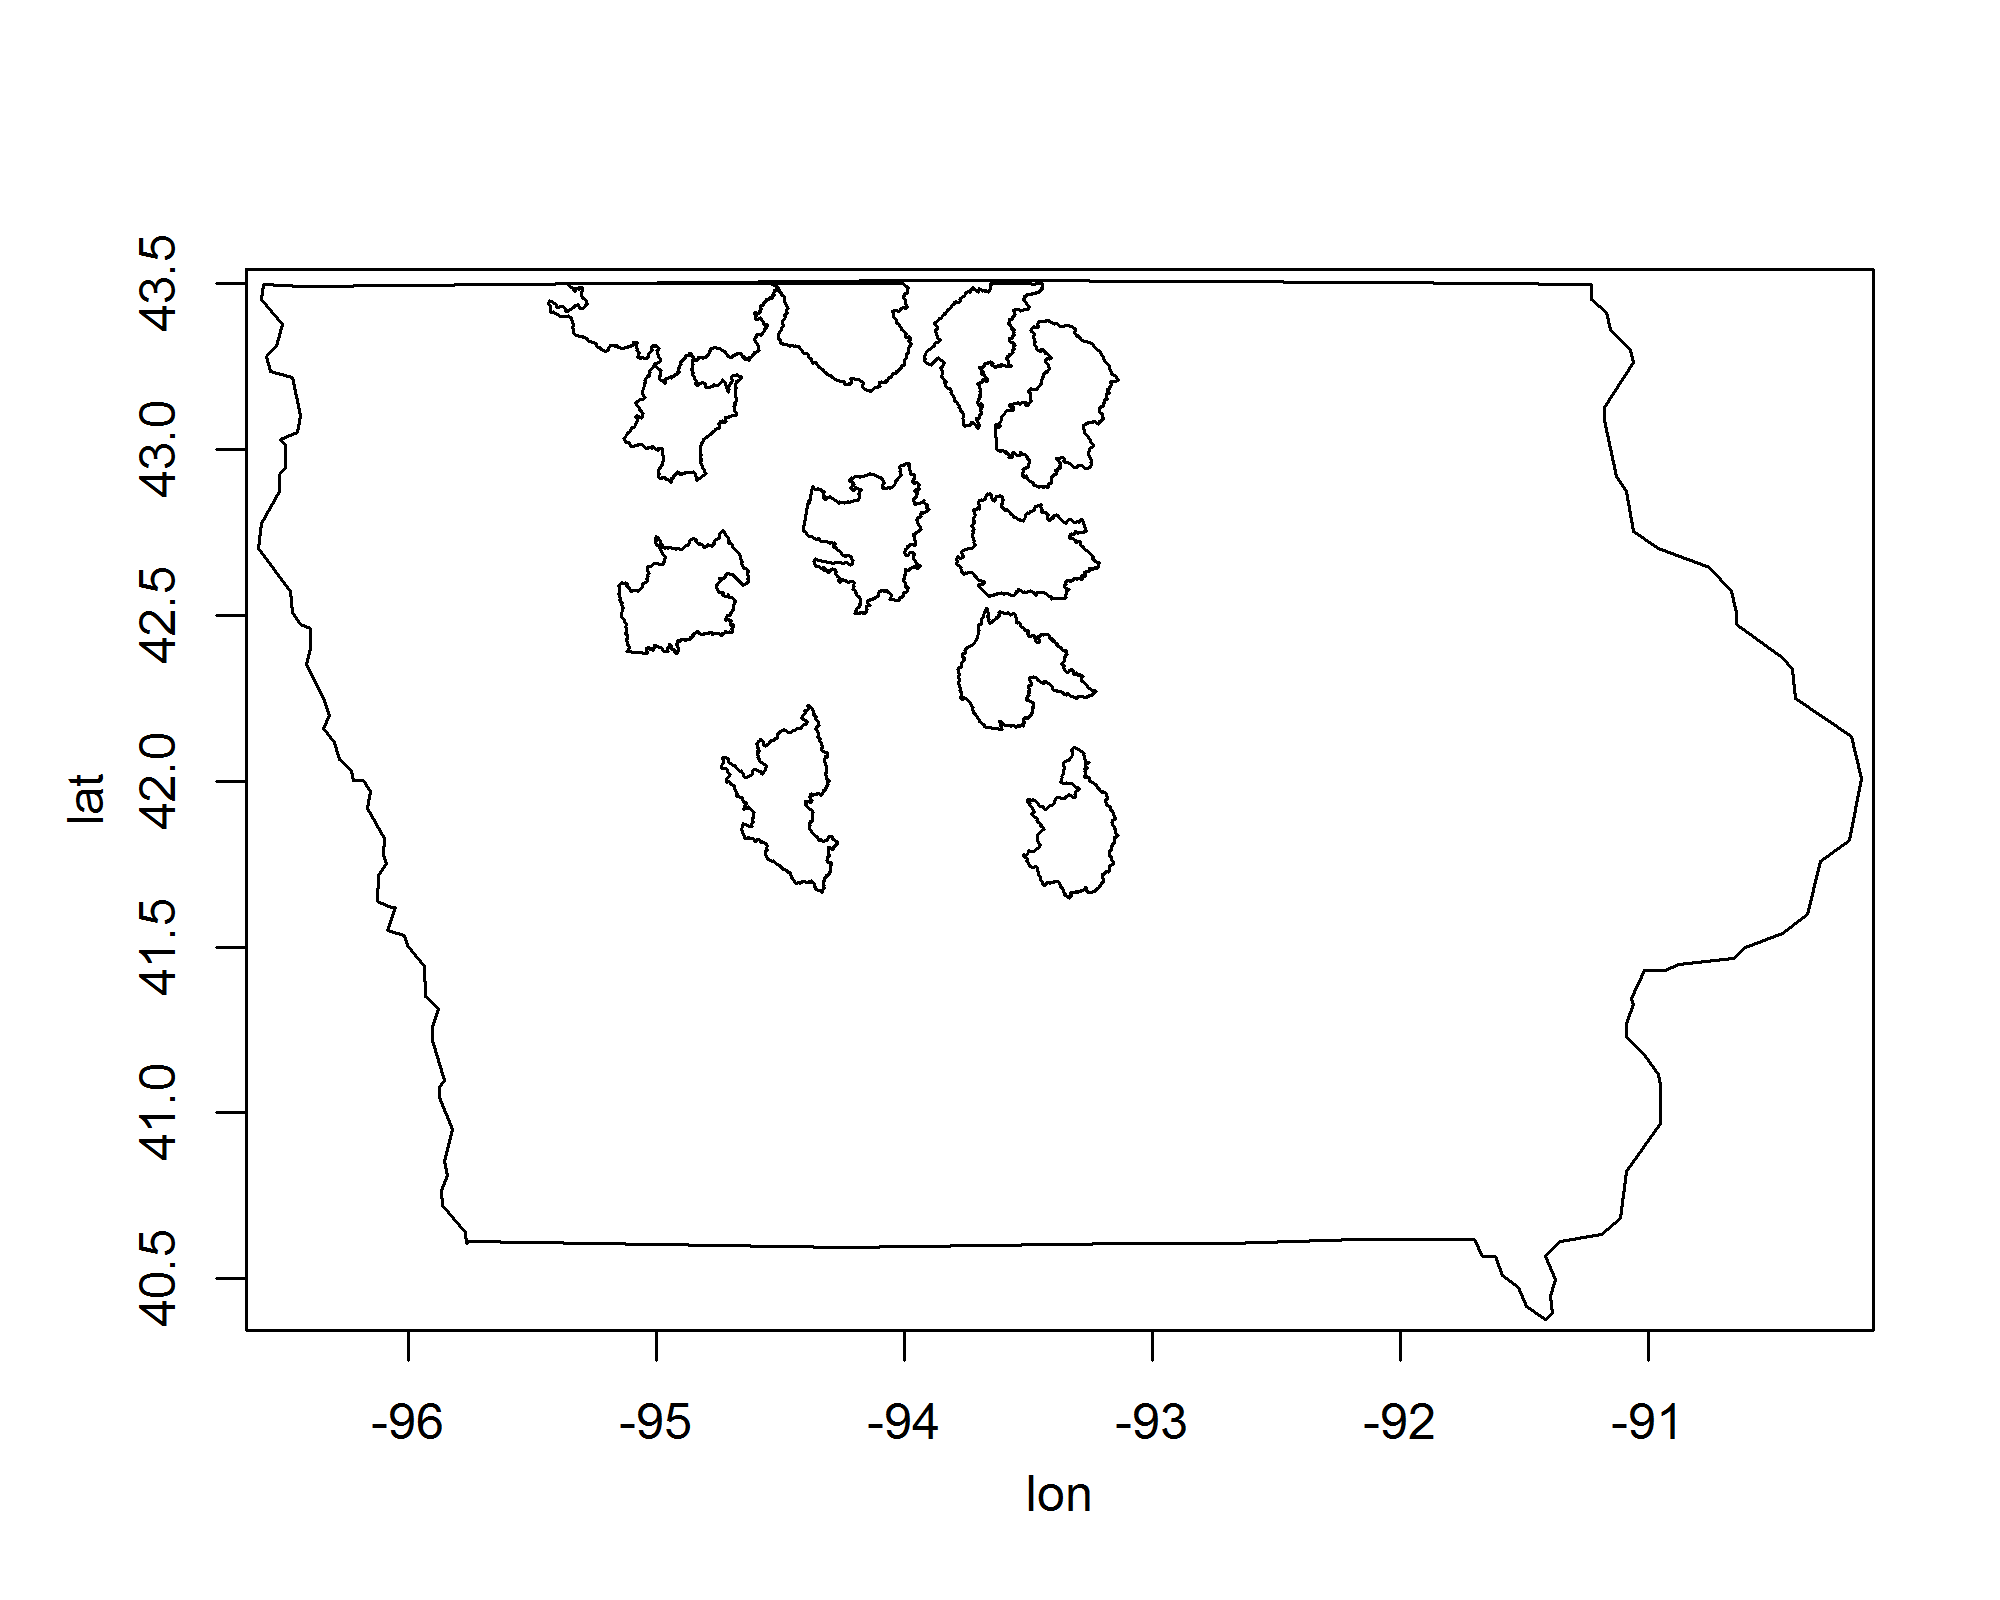
\includegraphics{mapfig}
   \caption{An example spatial dataset from ScienceBase, 
   visualized on top of the outline for the state of Iowa}
   \label{figure:iowafig}
 \end{figure}


\subsection{Search API}
\begin{itemize}
	\item{Go over general search API}
	\item{Free text search}
	\item{dateRange query}
	\item{Spatial query}
	\item{Hierarchical SB queries (sub-items)}
	\item{Combination of above}
\end{itemize}

\subsection{ScienceBase authentication}
ScienceBase has a large collection of open, reusable datasets and 
useful metadata. In addition to the public data available, ScienceBase
is also a platform for sharing and collaboration on private or in-progress 
data accessible through authenticated sessions. \pkg{sbtools} supports 
authentication to interact with access controlled items.

Authentication in \pkg{sbtools} is handled through the persistence of 
an authenticated session. By storing only the session, we do not need to 
store the plaintext password, which could represent a security issue. This
session state is persisted between function calls by the package. While  
expiration of the session can be difficult to predict, \pkg{sbtools}
makes a best effort to supply the user with meaningful error messages.

The authentication function \code{authenticate\_sb()} can accept a username
and password. Alternatively, to prevent plaintext passwords in R history, 
the password can be omitted and will be requested by R interactively. 
Authentication is persisted by the package, allowing for a single sign-in
and no tracking of usernames, passwords, or sessions during interactive or
script-based use. 

%Authentication in sbtools
\begin{example}
#to start an authenticated session
> authenticate_sb('username@usgs.gov')
> is_logged_in()
[1] TRUE
> session_logout()
> is_logged_in()
[1] FALSE
\end{example}

Most functions in \pkg{sbtools} can be used both anonymously and when
authenticated. This includes all query and data retrieval functions. 
When authenticated, these functions may return different results or fail
depending on the specific task. For example, when trying to access 
a private item using \code{item\_get()}, you must be authenticated, otherwise
it will throw and error ScienceBase does not differentiate between a missing
item and an item you don't have permission to access. Search follows a similar
pattern. When querying items with \code{query\_sb()}, public items are always 
visible while private items are not visible unless authenticated. 

\begin{example}
#Attempt to get a private item
> item_get('55de0027e4b0518e354dfcf0')
 Error: Item not found for ID=55de0027e4b0518e354dfcf0. Either the 
 item does not exist or the item is secured and requires authentication to access. 

#Get private item while authenticated
> authenticate_sb('username@usgs.gov')
> item_get('55de0027e4b0518e354dfcf0')
 <ScienceBase Item> 
  Title: Example Private Item
  Creator/LastUpdatedBy:     username@usgs.gov / username@usgs.gov
  Provenance (Created / Updated):  2015-08-26T18:06:31Z / 2015-12-30T14:59:27Z
  Children: FALSE
  Item ID: 55de0027e4b0518e354dfcf0
  Parent ID: 54257d8fe4b0e641df8b50af
  
#search expands to include user's private items when authenticated
#query while authenticated
> query_sb(list(q='username@usgs.gov'))
 <ScienceBase Item> 
  Title: Example Private Item
  Creator/LastUpdatedBy:     username@usgs.gov / username@usgs.gov
  Provenance (Created / Updated):  2015-08-26T18:06:31Z / 2015-12-30T14:59:27Z
  Children: FALSE
  Item ID: 55de0027e4b0518e354dfcf0
  Parent ID: 54257d8fe4b0e641df8b50af
  
> session_logout()
> query_sb(list(q='username@usgs.gov'))
list()
\end{example}

%Examples of authentication and other auth-related functions (check and such)

\subsection{Data editing and upload API}
For authenticated users, \pkg{sbtools} has functionality to support 
the full data lifecycle. This includes the creation, editing and removal
of items. Because item editing and creation cannot be done anonymously, 
this functionality only works while authenticated.

When we create new items, the only required inputs are "Parent Item" and "title". All 
items must have a non-empty title and a parent item. ScienceBase makes basic item creation
easy as all users have a personal home folder (called "My Items" on ScienceBase) and by default,
new items are created with that parent. The funciton \code{user\_id()} retrieves the
unique identifier for the user's home folder. 

\begin{example}
#create new item, by default under "My Items" parent
> new_item = item_create(title='new test item')
> new_item
<ScienceBase Item> 
  Title: new test item
  Creator/LastUpdatedBy:     username@usgs.gov / username@usgs.gov
  Provenance (Created / Updated):  2016-01-27T19:48:28Z / 2016-01-27T19:48:28Z
  Children: FALSE
  Item ID: 56a91f0ce4b0b28f1184dda8
  Parent ID: 54257d8fe4b0e641df8b50af
\end{example}

Once an item is created, we can edit the metadata or attach data files to that 
item using \pkg{sbtools}. 

\begin{example}
#giving the item a new title
> edited_item = item_update(new_item, list(title='new updated item'))
> edited_item
<ScienceBase Item> 
  Title: new updated item
  Creator/LastUpdatedBy:     lwinslow@usgs.gov / lwinslow@usgs.gov
  Provenance (Created / Updated):  2016-01-27T19:48:28Z / 2016-01-27T19:50:21Z
  Children: FALSE
  Item ID: 56a91f0ce4b0b28f1184dda8
  Parent ID: 54257d8fe4b0e641df8b50af

#appending files to item
> item_list_files(new_item)
data frame with 0 columns and 0 rows

> item_append_files(edited_item, 'test.dat')
> item_list_files(edited_item)
      fname size     url
1 README.md 1282     https://www.sciencebase.gov/[long URL truncated]


\end{example}

A full set of functions is also provided to modify and delete attached 
files and delete items. 

\begin{example}
#files can be selectively replaced with files of the same name
> item_list_files(edited_item)
      fname size     url
1 README.md 1282     https://www.sciencebase.gov/[long URL truncated]

# all=FALSE replaces files one by one, otherwise all files are removed
# before uploading the new files
> item_replace_files(new_item, 'README.md', all = FALSE)
> item_list_files(edited_item)
      fname size     url
1 README.md 608     https://www.sciencebase.gov/[long URL truncated]

#our item is easily deleted as well (use with caution, there is no confirmation)
> item_rm(edited_item)

> item_get(edited_item)
Error: Item not found for ID=56a91f0ce4b0b28f1184dda8. Either the item does 
not exist or the item is secured and requires authentication to access.
\end{example}


\subsection{SB Item identifiers}
One advanced and useful feature ScienceBase has is the ability to assign any 
number of custom item identifiers to items. The custom identifiers are made up 
of three parts: Scheme, Type and Key. Combined, these create a unique identifier. 
There are some standard Schemes used in ScienceBase. For example, DOIs (Digital 
Object Identifier) are stored as item identifiers with the scheme 
"https://www.sciencebase.gov/vocab/category/item/identifier" and type "DOI". 

\pkg{sbtools} can edit and query custom item identifiers using two functions:
\code{item\_update\_identifier} and \code{query\_item\_identifier}. 

\begin{example}
#create two items and assign custom identifiers
> ident_item = item_create(title='test data')
> item_update_identifier(ident_item, scheme='proj2', type='data', key='dataset1')
> ident_item = item_create(title='test publication')
> item_update_identifier(ident_item, scheme='proj2', type='publication', key='pdf1')

#query for created item
> query_item_identifier(scheme='proj2', type='publication', key='pdf1')
             title                       id
1 test publication 56a9371ee4b012c193aa3d65

\end{example}

The three-part identifier can be especially useful as a way to organize and 
access project data. All three parts can be quieried to access specific items 
directly. But the hierarchical nature can be used to query groups of items as well. 
For example, all items within the same project could be created with the same 
scheme. More specifically, a project might have multiple types of items, giving
users the ability to query items based on the project and category.

\begin{example}
#query all items in 'proj2'
> query_item_identifier(scheme='proj2')
             title                       id
1 test publication 56a9371ee4b012c193aa3d65
2        test data 56a93777e4b012c193aa3d68

#query just data items for a project
> query_item_identifier(scheme='proj2', type='data')
      title                       id
1 test data 56a93777e4b012c193aa3d68

\end{example}


